\documentclass[a4paper,11pt]{article}
\usepackage{amsmath,amsthm,amsfonts,amssymb,amscd,amstext,vmargin,graphics,graphicx,tabularx,multicol} \usepackage[french]{babel}
\usepackage[utf8]{inputenc}  
\usepackage[T1]{fontenc} 
\usepackage[T1]{fontenc}
\usepackage{amsmath,amssymb}
\usepackage{pstricks-add,tikz,tkz-tab,variations}
\usepackage[autolanguage,np]{numprint} 
\usepackage{color}
\usepackage{ulem}

\setmarginsrb{1.5cm}{0.5cm}{1cm}{0.5cm}{0cm}{0cm}{0cm}{0cm} %Gauche, haut, droite, haut
\newcounter{numexo}
\newcommand{\exo}[1]{\stepcounter{numexo}\noindent{\bf Exercice~\thenumexo} : \marginpar{\hfill /#1}}
\reversemarginpar


\newcounter{enumtabi}
\newcounter{enumtaba}
\newcommand{\q}{\stepcounter{enumtabi} \theenumtabi.  }
\newcommand{\qa}{\stepcounter{enumtaba} (\alph{enumtaba}) }
\newcommand{\initq}{\setcounter{enumtabi}{0}}
\newcommand{\initqa}{\setcounter{enumtaba}{0}}

\newcommand{\be}{\begin{enumerate}}
\newcommand{\ee}{\end{enumerate}}
\newcommand{\bi}{\begin{itemize}}
\newcommand{\ei}{\end{itemize}}
\newcommand{\bp}{\begin{pspicture*}}
\newcommand{\ep}{\end{pspicture*}}
\newcommand{\bt}{\begin{tabular}}
\newcommand{\et}{\end{tabular}}
\renewcommand{\tabularxcolumn}[1]{>{\centering}m{#1}} %(colonne m{} centrée, au lieu de p par défault) 
\newcommand{\tnl}{\tabularnewline}

\newcommand{\trait}{\noindent \rule{\linewidth}{0.2mm}}
\newcommand{\hs}[1]{\hspace{#1}}
\newcommand{\vs}[1]{\vspace{#1}}

\newcommand{\N}{\mathbb{N}}
\newcommand{\Z}{\mathbb{Z}}
\newcommand{\R}{\mathbb{R}}
\newcommand{\C}{\mathbb{C}}
\newcommand{\Dcal}{\mathcal{D}}
\newcommand{\Ccal}{\mathcal{C}}
\newcommand{\mc}{\mathcal}

\newcommand{\vect}[1]{\overrightarrow{#1}}
\newcommand{\ds}{\displaystyle}
\newcommand{\eq}{\quad \Leftrightarrow \quad}
\newcommand{\vecti}{\vec{\imath}}
\newcommand{\vectj}{\vec{\jmath}}
\newcommand{\Oij}{(O;\vec{\imath}, \vec{\jmath})}
\newcommand{\OIJ}{(O;I,J)}

\newcommand{\bmul}[1]{\begin{multicols}{#1}}
\newcommand{\emul}{\end{multicols}}


\newcommand{\reponse}[1][1]{%
\multido{}{#1}{\makebox[\linewidth]{\rule[0pt]{0pt}{20pt}\dotfill}
}}

\newcommand{\titre}[5] 
% #1: titre #2: haut gauche #3: bas gauche #4: haut droite #5: bas droite
{
\noindent #2 \hfill #4 \\
#3 \hfill #5

\vspace{-1.6cm}

\begin{center}\rule{6cm}{0.5mm}\end{center}
\vspace{0.2cm}
\begin{center}{\large{\textbf{#1}}}\end{center}
\begin{center}\rule{6cm}{0.5mm}\end{center}
}



\begin{document}
\pagestyle{empty}
\titre{Contrôle 1}{Nom}{Prénom}{Date}{Classe}
\vspace*{0.5cm}


\begin{flushleft}
\begin{tabular}{|m{6cm}|m{2.5cm}|m{2.5cm}|m{2.5cm}|m{2.5cm}|}
\hline 
\textbf{Compétences} & \begin{center}
\textbf{Très bonne maîtrise}
\end{center} & \begin{center}
\textbf{Maîtrise satisfaisante}
\end{center}  & \begin{center}
\textbf{Maîtrise faible}
\end{center} & \begin{center}
\textbf{Maîtrise insuffisante}
\end{center} \\ 
\hline 
Je dois savoir décomposer un problème en sous-problèmes &  &  & &\\
\hline
Je dois connaître et utiliser les puissances dans les calculs, savoir donner l'écriture scientifique d'un nombre&  &  & & \\ 
\hline
Je dois savoir analyser et étudier les sections de certains solides par un plan &  &  &  &\\ 
\hline 


\end{tabular} 
\end{flushleft}

\vspace*{0.75cm}

\exo{3} Écrire les expressions suivantes sous la forme d'une seule puissance.\\



$J = 3^{7} \times 3^{-2}$ \hspace*{1.5cm} $L = \dfrac{8^{3}}{8^{5}}$ \hspace*{1.5cm} 	$O = (2^{3})^{4} \times 2^{-2} \times (2^{-1})^{3}$ \hspace*{1.5cm} $M = \dfrac{(10^{-3})^{2} \times 10^{-1}}{10^{-5}}$\\

\vspace*{1cm}


\exo{2.5} On donne $C = \dfrac{10^{5} \times 42 \times 10^{-12}}{0,7 \times 10^{10}}$, \hspace*{0.5cm} $D= 0,0082 \times 10^{-3}$ \hspace*{0.5cm} et \hspace*{0.5cm} $E = 56 379,65 \times 10^{3}$.\\

\vspace*{0.5cm}

$\rightarrow$ Écrire les expressions C, D et E sous forme scientifique. (Détailler les étapes de calculs pour l'expression C.)\\

\vspace*{0.75cm}

\exo{4} 
\bmul{2}

A partir des information portées sur le dessin suivant, démontrer que les droites (EF) et (FG) sont perpendiculaires.

\columnbreak

\includegraphics[scale=1]{difficicel.eps} 


\emul


\vspace*{0.2cm}

\exo{1.5} Calculer le volume des solides suivants.\\

\qa \hspace*{7cm} \qa
 
\includegraphics[scale=1]{volprismedroit.eps} \hspace*{2.5cm}  \includegraphics[scale=0.65]{cylindrevol.eps} 

\newpage

\vspace*{0.3cm}

\exo{5.5}

\begin{center}
\includegraphics[scale=1]{exoespace1.eps} 
\end{center}

ABCDEFGH est un parallélépipède rectangle tel que AE = 3 m, AD = 4 m et AB = 6 m.\\

\q Représenter sur le sujet, la section AEGC du pavé droite parallèle à l'arête [GC].\\




\vspace*{0.5cm}

\q Quelle est la nature de cette section ? En déduire la nature du triangle EGC.\\

\q Calculer la valeur exacte de la diagonale [EC] de ce parallélépipède rectangle.\\

\q Calculer le volume de ABCDEFGH ?\\

\vspace*{0.5cm}

\exo{4}\\

M. Dupond et M. Durand ont chacun une entreprise de 100 personnes. Nous avons les informations suivantes :\\

\begin{tabular}{|c|c|c|}
\hline 
Âge moyen & M. Dupond & M. Durand \\ 
\hline 
Hommes  & 51 & 54 \\ 
\hline 
Femmes & 36 & 39 \\ 
\hline 
\end{tabular} \hspace*{2.25cm} \begin{tabular}{|c|c|c|}
\hline 
Effectif & M. Dupond & M. Durand \\ 
\hline 
Hommes  & 50 & 20 \\ 
\hline 
Femmes & 50 & 80 \\ 
\hline 
\end{tabular} \\

\vspace*{0.5cm}

\initq \q A l'aide des tableaux ci-dessus, décrire en 2 phrases la composition de l'entreprise de M. Durand.\\

\q Hugo dit à son frère : " En moyenne, les personnes de l'entreprise de M. Durand sont plus vieille que celles de l'entreprise de M. Dupond.\\
Qu'en pensez-vous ?\\

\textit{Toute trace de recherche, même incomplète, ou d'initiative même infructueuse, sera prise en compte dans l'évaluation.}







\end{document}
